\begin{proofbox}
\textbf{\textcolor{CProof}{统一条件与记号}}
设 $p\ne0$，$A(x_1,y_1)$、$B(x_2,y_2)$ 是 $y^2=2px$ 上两个不同点，
过 $A,B$ 的切线交于 $M(x_M,y_M)$，弦 $AB$ 中点为 $N(x_N,y_N)$。
因为
\[
 x_1=\frac{y_1^2}{2p},\qquad x_2=\frac{y_2^2}{2p},
\]
若 $y_1=y_2$，则 $x_1=x_2$，与 $A\ne B$ 矛盾。
因此下文始终可以使用
\[\boxed{y_1-y_2\ne0}.\]
任意切点 $T(x_0,y_0)$ 处的切线为 $yy_0=p(x+x_0)$。
这条直线与抛物线联立后得到 $(y-y_0)^2=0$，故只有一个公共点 $T$。
整个证明不需要使用导数。

\medskip
\par\noindent\begin{minipage}{\linewidth}
\textbf{\textcolor{CProof}{方法一｜门槛最低：切线相减＋平方差＋中点公式}}
\begin{center}
\begingroup
\def\Cmode{1}
% Exact model: p=2, A=(1,-2), B=(4,4), M=(-2,1), N=(5/2,1).
\begin{tikzpicture}[x=1.15cm,y=0.85cm,>=stealth,font=\small]
\path[use as bounding box] (-3.1,-3.5) rectangle (6.1,5.2);
\draw[->,gray] (-2.9,0)--(5.7,0) node[right] {$x$};
\draw[->,gray] (0,-2.8)--(0,4.9) node[above] {$y$};
\node[below left] at (0,0) {$O$};
\draw[blue,thick,domain=-2.5:4.5,samples=100] plot ({\x*\x/4},\x);
\node[blue,right] at (5.1,4.2) {$y^2=4x$};
\draw[orange,thick] (-2.6,1.6)--(1.6,-2.6);
\draw[orange,thick] (-2.6,.7)--(5,4.5);
\draw[gray,thick] (1,-2)--(4,4);
\draw[red,very thick] (-2,1)--(2.5,1);
\ifnum\Cmode=1
  \draw[dashed,gray] (1,-2)--(-.55,-2) (4,4)--(-.55,4);
  \draw[<->,blue] (-.55,-2)--(-.55,1) node[midway,left,fill=white,inner sep=2pt] {$3$};
  \draw[<->,blue] (-.55,1)--(-.55,4) node[midway,left,fill=white,inner sep=2pt] {$3$};
  \fill[red] (0,1) circle (2pt) node[above left=2pt] {$H$};
\fi
\ifnum\Cmode=2
  \draw[dashed,blue] (1,-2)--(4,-2)--(4,4);
  \node[below,blue] at (2.5,-2.7) {$\Delta x=3$};
  \node[right,blue,fill=white,inner sep=2pt] at (4,-.6) {$\Delta y=6$};
  \node[fill=white,inner sep=3pt] at (2.8,4.85) {$AB:\ x=\tfrac12y+2,\quad pt=1$};
\fi
\ifnum\Cmode=3
  \node[fill=white,inner sep=3pt] at (2.7,4.85) {$AB:\ y=2(x-2)$};
  \node[anchor=west,fill=white,inner sep=3pt] at (3.4,2) {$y_1=-2,\ y_2=4$};
\fi
\ifnum\Cmode=4
  \draw[dashed,red] (-2,1)--(-2,-.7) (2.5,1)--(2.5,-.7);
  \draw[<->,red] (-2,-.6)--(2.5,-.6) node[pos=1,below right,fill=white,inner sep=3pt] {$x_N-x_M=\tfrac92>0$};
\fi
\fill (1,-2) circle (2pt) node[right=10pt] {$A(1,-2)$};
\fill (4,4) circle (2pt) node[above left] {$B(4,4)$};
\fill[red] (-2,1) circle (2pt) node[below left] {$M(-2,1)$};
\fill[red] (2.5,1) circle (2pt) node[below right,fill=white,inner sep=2pt] {$N(\tfrac52,1)$};
\ifnum\Cmode=0
  \node[red,above,fill=white,inner sep=3pt] at (.6,1) {$y_M=y_N=1$};
\fi
\end{tikzpicture}

\endgroup


观察 $H$ 把两切点的高度差平分；本法用切线相减求出 $M$ 的这一高度。
\end{center}
\end{minipage}\par

\begin{description}[style=nextline,leftmargin=2.8em,labelsep=0.5em,itemsep=0.5em]
\item[\textbf{第 1 步：写出两条切线。}]
由于 $A,B$ 分别在抛物线上，
\[
 \begin{cases}
 y_1y=p(x+x_1),\\
 y_2y=p(x+x_2).
 \end{cases}
\]
它们交于 $M$，所以把交点坐标代进去：
\[
 \begin{cases}
 y_1y_M=p(x_M+x_1),\\
 y_2y_M=p(x_M+x_2).
 \end{cases}
\]
\textbf{为什么这样做？}两式都有 $x_M$，相减后它会消失，只剩下需要的 $y_M$。

\item[\textbf{第 2 步：两式相减，消去 $x_M$。}]
将第一式减去第二式，逐项计算：
\[
\begin{aligned}
 y_1y_M-y_2y_M
 &=p(x_M+x_1)-p(x_M+x_2)\\
 & =p(x_1-x_2).
\end{aligned}
\]
提出公因式得
\[ (y_1-y_2)y_M=p(x_1-x_2). \]

\item[\textbf{第 3 步：利用抛物线方程，把横坐标差变成平方差。}]
由于 $x_i=y_i^2/(2p)$，
\[
\begin{aligned}
 (y_1-y_2)y_M
 &=p\left(\frac{y_1^2}{2p}-\frac{y_2^2}{2p}\right)\\
 &=\frac{y_1^2-y_2^2}{2}\\
 &=\frac{(y_1-y_2)(y_1+y_2)}{2}.
\end{aligned}
\]
因 $y_1-y_2\ne0$，两边同时除以它，得到
\[\boxed{y_M=\frac{y_1+y_2}{2}}.\]
\textbf{为什么会有平均数？}平方差拆成“差乘和”，约去同一个“差”，留下的正是“和的一半”。

\item[\textbf{第 4 步：求弦中点，比较高度。}]
中点坐标公式给出
\[
 N\left(\frac{x_1+x_2}{2},\frac{y_1+y_2}{2}\right),\qquad
 y_N=\frac{y_1+y_2}{2}=y_M.
\]
故 $M,N$ 的高度相同，$MN$ 水平；是否与 $x$ 轴平行还是重合，要看这个共同的纵坐标是否为零。
\end{description}

\medskip
\par\noindent\begin{minipage}{\linewidth}
\textbf{\textcolor{CProof}{方法二｜速度最快：已知弦方程时直接比较两个“平均高度”}}
\begin{center}
\begingroup
\def\Cmode{2}
% Exact model: p=2, A=(1,-2), B=(4,4), M=(-2,1), N=(5/2,1).
\begin{tikzpicture}[x=1.15cm,y=0.85cm,>=stealth,font=\small]
\path[use as bounding box] (-3.1,-3.5) rectangle (6.1,5.2);
\draw[->,gray] (-2.9,0)--(5.7,0) node[right] {$x$};
\draw[->,gray] (0,-2.8)--(0,4.9) node[above] {$y$};
\node[below left] at (0,0) {$O$};
\draw[blue,thick,domain=-2.5:4.5,samples=100] plot ({\x*\x/4},\x);
\node[blue,right] at (5.1,4.2) {$y^2=4x$};
\draw[orange,thick] (-2.6,1.6)--(1.6,-2.6);
\draw[orange,thick] (-2.6,.7)--(5,4.5);
\draw[gray,thick] (1,-2)--(4,4);
\draw[red,very thick] (-2,1)--(2.5,1);
\ifnum\Cmode=1
  \draw[dashed,gray] (1,-2)--(-.55,-2) (4,4)--(-.55,4);
  \draw[<->,blue] (-.55,-2)--(-.55,1) node[midway,left,fill=white,inner sep=2pt] {$3$};
  \draw[<->,blue] (-.55,1)--(-.55,4) node[midway,left,fill=white,inner sep=2pt] {$3$};
  \fill[red] (0,1) circle (2pt) node[above left=2pt] {$H$};
\fi
\ifnum\Cmode=2
  \draw[dashed,blue] (1,-2)--(4,-2)--(4,4);
  \node[below,blue] at (2.5,-2.7) {$\Delta x=3$};
  \node[right,blue,fill=white,inner sep=2pt] at (4,-.6) {$\Delta y=6$};
  \node[fill=white,inner sep=3pt] at (2.8,4.85) {$AB:\ x=\tfrac12y+2,\quad pt=1$};
\fi
\ifnum\Cmode=3
  \node[fill=white,inner sep=3pt] at (2.7,4.85) {$AB:\ y=2(x-2)$};
  \node[anchor=west,fill=white,inner sep=3pt] at (3.4,2) {$y_1=-2,\ y_2=4$};
\fi
\ifnum\Cmode=4
  \draw[dashed,red] (-2,1)--(-2,-.7) (2.5,1)--(2.5,-.7);
  \draw[<->,red] (-2,-.6)--(2.5,-.6) node[pos=1,below right,fill=white,inner sep=3pt] {$x_N-x_M=\tfrac92>0$};
\fi
\fill (1,-2) circle (2pt) node[right=10pt] {$A(1,-2)$};
\fill (4,4) circle (2pt) node[above left] {$B(4,4)$};
\fill[red] (-2,1) circle (2pt) node[below left] {$M(-2,1)$};
\fill[red] (2.5,1) circle (2pt) node[below right,fill=white,inner sep=2pt] {$N(\tfrac52,1)$};
\ifnum\Cmode=0
  \node[red,above,fill=white,inner sep=3pt] at (.6,1) {$y_M=y_N=1$};
\fi
\end{tikzpicture}

\endgroup


图取 $p=2$：$t=\Delta x/\Delta y=3/6=1/2$，因此 $M,N$ 的高度均为 $pt=1$。
\end{center}
\end{minipage}\par
\textbf{适用信号：}题目给出或容易求得弦 $AB$ 的方程。
因为 $y_1\ne y_2$，弦 $AB$ 一定能写成
\[
\boxed{x=ty+q},\qquad t=\frac{x_2-x_1}{y_2-y_1}.
\]
\textbf{说明：}$t$ 是 $x$ 的变化量除以 $y$ 的变化量，所以\textbf{竖直弦 $x=q$ 也包含在内}（此时 $t=0$）。

\begin{description}[style=nextline,leftmargin=2.8em,labelsep=0.5em,itemsep=0.5em]
\item[\textbf{第 1 步：由弦方程快速找到中点高度。}]
将 $x=ty+q$ 代入 $y^2=2px$：
\[
 y^2=2p(ty+q)
 \quad\Longleftrightarrow\quad y^2-2pty-2pq=0.
\]
这个一元二次方程的两个根就是 $A,B$ 的纵坐标 $y_1,y_2$。
由一元二次方程两根之和的公式，
\[
 y_1+y_2=2pt,
 \qquad\boxed{y_N=\frac{y_1+y_2}{2}=pt}.
\]

\item[\textbf{第 2 步：由切线相减快速找到交点高度。}]
两条切线在 $M$ 处满足
\[
 y_M(y_1-y_2)=p(x_1-x_2).
\]
又因 $A,B$ 都在 $x=ty+q$ 上，所以 $x_1-x_2=t(y_1-y_2)$。
代入、再约去 $y_1-y_2\ne0$：
\[
 \boxed{y_M=pt=y_N}.
\]
\end{description}
\textbf{考场速用：}若弦已写成 $x=ty+q$，可直接写 $y_M=y_N=pt$；
若题目要求证明，则补上上面两步依据。

\medskip
\par\noindent\begin{minipage}{\linewidth}
\textbf{\textcolor{CProof}{方法三｜步骤最少：切点弦方程＋一元二次方程两根之和}}
\begin{center}
\begingroup
\def\Cmode{3}
% Exact model: p=2, A=(1,-2), B=(4,4), M=(-2,1), N=(5/2,1).
\begin{tikzpicture}[x=1.15cm,y=0.85cm,>=stealth,font=\small]
\path[use as bounding box] (-3.1,-3.5) rectangle (6.1,5.2);
\draw[->,gray] (-2.9,0)--(5.7,0) node[right] {$x$};
\draw[->,gray] (0,-2.8)--(0,4.9) node[above] {$y$};
\node[below left] at (0,0) {$O$};
\draw[blue,thick,domain=-2.5:4.5,samples=100] plot ({\x*\x/4},\x);
\node[blue,right] at (5.1,4.2) {$y^2=4x$};
\draw[orange,thick] (-2.6,1.6)--(1.6,-2.6);
\draw[orange,thick] (-2.6,.7)--(5,4.5);
\draw[gray,thick] (1,-2)--(4,4);
\draw[red,very thick] (-2,1)--(2.5,1);
\ifnum\Cmode=1
  \draw[dashed,gray] (1,-2)--(-.55,-2) (4,4)--(-.55,4);
  \draw[<->,blue] (-.55,-2)--(-.55,1) node[midway,left,fill=white,inner sep=2pt] {$3$};
  \draw[<->,blue] (-.55,1)--(-.55,4) node[midway,left,fill=white,inner sep=2pt] {$3$};
  \fill[red] (0,1) circle (2pt) node[above left=2pt] {$H$};
\fi
\ifnum\Cmode=2
  \draw[dashed,blue] (1,-2)--(4,-2)--(4,4);
  \node[below,blue] at (2.5,-2.7) {$\Delta x=3$};
  \node[right,blue,fill=white,inner sep=2pt] at (4,-.6) {$\Delta y=6$};
  \node[fill=white,inner sep=3pt] at (2.8,4.85) {$AB:\ x=\tfrac12y+2,\quad pt=1$};
\fi
\ifnum\Cmode=3
  \node[fill=white,inner sep=3pt] at (2.7,4.85) {$AB:\ y=2(x-2)$};
  \node[anchor=west,fill=white,inner sep=3pt] at (3.4,2) {$y_1=-2,\ y_2=4$};
\fi
\ifnum\Cmode=4
  \draw[dashed,red] (-2,1)--(-2,-.7) (2.5,1)--(2.5,-.7);
  \draw[<->,red] (-2,-.6)--(2.5,-.6) node[pos=1,below right,fill=white,inner sep=3pt] {$x_N-x_M=\tfrac92>0$};
\fi
\fill (1,-2) circle (2pt) node[right=10pt] {$A(1,-2)$};
\fill (4,4) circle (2pt) node[above left] {$B(4,4)$};
\fill[red] (-2,1) circle (2pt) node[below left] {$M(-2,1)$};
\fill[red] (2.5,1) circle (2pt) node[below right,fill=white,inner sep=2pt] {$N(\tfrac52,1)$};
\ifnum\Cmode=0
  \node[red,above,fill=white,inner sep=3pt] at (.6,1) {$y_M=y_N=1$};
\fi
\end{tikzpicture}

\endgroup


图取 $M(-2,1),p=2$：切点弦为 $y=2(x-2)$，两交点纵坐标为 $-2,4$，和为 $2y_M=2$。
\end{center}
\end{minipage}\par
\textbf{前置结论：}过 $A,B$ 的切线交于 $M(x_M,y_M)$ 时，直线 $AB$ 的方程为
\[
\boxed{y_My=p(x+x_M)}.
\]
\textbf{为什么这就是 $AB$？}在切点 $A$ 处的切线公式是
$y_1y_M=p(x_1+x_M)$，在 $B$ 处同样有
$y_2y_M=p(x_2+x_M)$。因此 $A,B$ 都满足上面的直线方程；又因 $A\ne B$，这条直线就是 $AB$。

\begin{description}[style=nextline,leftmargin=2.8em,labelsep=0.5em,itemsep=0.5em]
\item[\textbf{第 1 步：联立弦方程与抛物线。}]
由 $y_My=p(x+x_M)$ 得
\[
 x=\frac{y_M}{p}y-x_M.
\]
代入 $y^2=2px$ 得
\[
\boxed{y^2-2y_My+2px_M=0}.
\]

\item[\textbf{第 2 步：直接用两根之和。}]
这个方程的两个根为 $y_1,y_2$，因此
\[
 y_1+y_2=2y_M
 \quad\Longrightarrow\quad
 \boxed{y_N=\frac{y_1+y_2}{2}=y_M}.
\]
\end{description}
\textbf{几何意义：}切点弦 $AB$ 与抛物线相交于 $A,B$，
而它的方程里直接出现 $y_M$；两根之和告诉我们，这个 $y_M$ 就是两切点的平均高度。
\textbf{提醒：}本法使用的是高中一元二次方程的两根之和；不需要其他概念。

\medskip
\par\noindent\begin{minipage}{\linewidth}
\textbf{\textcolor{CProof}{方法四｜常规通用：完整求出交点、中点及距离}}
\begin{center}
\begingroup
\def\Cmode{4}
% Exact model: p=2, A=(1,-2), B=(4,4), M=(-2,1), N=(5/2,1).
\begin{tikzpicture}[x=1.15cm,y=0.85cm,>=stealth,font=\small]
\path[use as bounding box] (-3.1,-3.5) rectangle (6.1,5.2);
\draw[->,gray] (-2.9,0)--(5.7,0) node[right] {$x$};
\draw[->,gray] (0,-2.8)--(0,4.9) node[above] {$y$};
\node[below left] at (0,0) {$O$};
\draw[blue,thick,domain=-2.5:4.5,samples=100] plot ({\x*\x/4},\x);
\node[blue,right] at (5.1,4.2) {$y^2=4x$};
\draw[orange,thick] (-2.6,1.6)--(1.6,-2.6);
\draw[orange,thick] (-2.6,.7)--(5,4.5);
\draw[gray,thick] (1,-2)--(4,4);
\draw[red,very thick] (-2,1)--(2.5,1);
\ifnum\Cmode=1
  \draw[dashed,gray] (1,-2)--(-.55,-2) (4,4)--(-.55,4);
  \draw[<->,blue] (-.55,-2)--(-.55,1) node[midway,left,fill=white,inner sep=2pt] {$3$};
  \draw[<->,blue] (-.55,1)--(-.55,4) node[midway,left,fill=white,inner sep=2pt] {$3$};
  \fill[red] (0,1) circle (2pt) node[above left=2pt] {$H$};
\fi
\ifnum\Cmode=2
  \draw[dashed,blue] (1,-2)--(4,-2)--(4,4);
  \node[below,blue] at (2.5,-2.7) {$\Delta x=3$};
  \node[right,blue,fill=white,inner sep=2pt] at (4,-.6) {$\Delta y=6$};
  \node[fill=white,inner sep=3pt] at (2.8,4.85) {$AB:\ x=\tfrac12y+2,\quad pt=1$};
\fi
\ifnum\Cmode=3
  \node[fill=white,inner sep=3pt] at (2.7,4.85) {$AB:\ y=2(x-2)$};
  \node[anchor=west,fill=white,inner sep=3pt] at (3.4,2) {$y_1=-2,\ y_2=4$};
\fi
\ifnum\Cmode=4
  \draw[dashed,red] (-2,1)--(-2,-.7) (2.5,1)--(2.5,-.7);
  \draw[<->,red] (-2,-.6)--(2.5,-.6) node[pos=1,below right,fill=white,inner sep=3pt] {$x_N-x_M=\tfrac92>0$};
\fi
\fill (1,-2) circle (2pt) node[right=10pt] {$A(1,-2)$};
\fill (4,4) circle (2pt) node[above left] {$B(4,4)$};
\fill[red] (-2,1) circle (2pt) node[below left] {$M(-2,1)$};
\fill[red] (2.5,1) circle (2pt) node[below right,fill=white,inner sep=2pt] {$N(\tfrac52,1)$};
\ifnum\Cmode=0
  \node[red,above,fill=white,inner sep=3pt] at (.6,1) {$y_M=y_N=1$};
\fi
\end{tikzpicture}

\endgroup


图中横向距离为 $5/2-(-2)=9/2$；本法求出完整坐标，再证此距离非零。
\end{center}
\end{minipage}\par
本法适用于题目要求交点坐标、长度或左右位置的情况。

\begin{description}[style=nextline,leftmargin=2.8em,labelsep=0.5em,itemsep=0.5em]
\item[\textbf{第 1 步：联立切线方程求 $y_M$。}]
\[
\begin{cases}
 y_1y_M=p(x_M+x_1),\\
 y_2y_M=p(x_M+x_2).
\end{cases}
\]
两式相减，并用 $x_i=y_i^2/(2p)$：
\[
 (y_1-y_2)y_M=\frac{y_1^2-y_2^2}{2}
 \quad\Longrightarrow\quad
 \boxed{y_M=\frac{y_1+y_2}{2}}.
\]

\item[\textbf{第 2 步：把 $y_M$ 代回一条切线，求 $x_M$。}]
由 $y_1y_M=p(x_M+x_1)$，
\[
\begin{aligned}
 px_M
 &=y_1y_M-px_1\\
 &=\frac{y_1(y_1+y_2)}2-\frac{y_1^2}{2}\\
 &=\frac{y_1y_2}{2}.
\end{aligned}
\]
因此
\[
\boxed{M\left(\frac{y_1y_2}{2p},\frac{y_1+y_2}{2}\right)}.
\]

\item[\textbf{第 3 步：直接求中点 $N$。}]
\[
\begin{aligned}
 x_N&=\frac{x_1+x_2}{2}
 =\frac{y_1^2+y_2^2}{4p},\\
 y_N&=\frac{y_1+y_2}{2}.
\end{aligned}
\]
因此
\[
\boxed{N\left(\frac{y_1^2+y_2^2}{4p},\frac{y_1+y_2}{2}\right)}.
\]

\item[\textbf{第 4 步：证明 $M,N$ 不重合，再判断位置。}]
\[
\begin{aligned}
 x_N-x_M
 &=\frac{y_1^2+y_2^2}{4p}-\frac{y_1y_2}{2p}\\
 &=\frac{y_1^2-2y_1y_2+y_2^2}{4p}\\
 &=\boxed{\frac{(y_1-y_2)^2}{4p}\ne0}.
\end{aligned}
\]
所以 $M\ne N$，而且两点纵坐标相同，故 $MN$ 是一条确定的水平直线。
由于是水平距离，
\[
\boxed{|MN|=|x_N-x_M|=\frac{(y_1-y_2)^2}{4|p|}}.
\]
当 $p>0$ 时 $x_N>x_M$（$N$ 在右），当 $p<0$ 时 $x_N<x_M$（$N$ 在左）。
若 $y_1+y_2=0$，$MN$ 与 $x$ 轴\textbf{重合}；否则才与 $x$ 轴\textbf{平行}。
\end{description}

\medskip
\par\noindent\begin{minipage}{\linewidth}
\textbf{\textcolor{CProof}{对称情形｜$x^2=2py$ 的完整验证}}
\begin{center}
\begin{tikzpicture}[x=1cm,y=1cm,>=stealth,font=\small]
\path[use as bounding box] (-3,-2.5) rectangle (5.1,4.6);
\draw[->,gray] (-2.8,0)--(4.8,0) node[right] {$x$};
\draw[->,gray] (0,-2.2)--(0,4.2) node[above] {$y$};
\node[below left] at (0,0) {$O$};
\draw[blue,thick,domain=-2.5:4,samples=90] plot (\x,{\x*\x/4});
\node[blue,right] at (3.8,3.5) {$x^2=4y$};
\draw[orange,thick] (-2.4,1.4)--(1.4,-2.4) (.8,-2.4)--(4,4);
\draw[gray,thick] (-2,1)--(4,4);
\draw[red,very thick] (1,-2)--(1,2.5);
\fill (-2,1) circle (2pt) node[below left=3pt] {$A(-2,1)$};
\fill (4,4) circle (2pt) node[above left] {$B(4,4)$};
\fill[red] (1,-2) circle (2pt) node[right] {$M(1,-2)$};
\fill[red] (1,2.5) circle (2pt) node[above left] {$N(1,\tfrac52)$};
\node[red,right,fill=white,inner sep=3pt] at (1,.7) {$x_M=x_N=1$};
\end{tikzpicture}


交换坐标后比较横坐标：$M,N$ 同在 $x=1$ 上，纵向间隔为 $9/2$。
\end{center}
\end{minipage}\par
现在设 $A(x_1,y_1),B(x_2,y_2)$ 在 $x^2=2py$ 上且 $A\ne B$。
同理有 $x_1\ne x_2$，$y_i=x_i^2/(2p)$。
两条切线在 $M$ 处满足
\[
\begin{cases}
 x_1x_M=p(y_M+y_1),\\
 x_2x_M=p(y_M+y_2).
\end{cases}
\]
相减消去 $y_M$：
\[
 (x_1-x_2)x_M=p(y_1-y_2)
 =\frac{x_1^2-x_2^2}{2}.
\]
所以
\[
\boxed{x_M=\frac{x_1+x_2}{2}=x_N}.
\]
再将 $x_M$ 代入第一条切线，
\[
py_M=x_1x_M-py_1
=\frac{x_1(x_1+x_2)}2-\frac{x_1^2}2
=\frac{x_1x_2}{2},
\]
从而
\[
\boxed{M\left(\frac{x_1+x_2}{2},\frac{x_1x_2}{2p}\right),\quad
N\left(\frac{x_1+x_2}{2},\frac{x_1^2+x_2^2}{4p}\right)}.
\]
\[
\boxed{y_N-y_M=\frac{(x_1-x_2)^2}{4p}\ne0,\qquad
|MN|=\frac{(x_1-x_2)^2}{4|p|}}.
\]
因此 $MN$ 竖直，若 $x_1+x_2\ne0$ 则与 $y$ 轴平行；
若 $x_1+x_2=0$ 则与 $y$ 轴重合。

\medskip
\textbf{\textcolor{CProof}{四种方法如何选择}}
初学者优先\textbf{方法一}；已经知道弦方程时优先\textbf{方法二}；
熟悉“切点弦方程＋两根之和”时\textbf{方法三步骤最少}；
同时要算交点完整坐标、距离和位置时使用\textbf{方法四}。
\end{proofbox}
